\subsection{Struktur des Modells}

Die Struktur des Modells für Erklärungen orientiert sich an den Forschungsfragen und Anforderungen an das Modell, Ergebnissen aus der Literaturrecherche sowie dem bestehenden Konzept der Qualitätsmodelle \cite{schneider2012abenteuer} (siehe \autoref{sec:basics_quality_models}).

In der Literatur wurden einige Aspekte des Modells nicht nur verschieden benannt, sondern auch zum Teil in Oberkategorien gegliedert oder auf verschiedenen Abstraktionsebenen betrachtet. Hieraus ergibt sich eine hierarchische Anordung des Modells. Verschiedene Abstraktionsebenen enthalten auch die von \citeauthor{schneider2012abenteuer} vorgestellten Qualitätsmodelle \cite{schneider2012abenteuer}. Dabei werden abstrakte Ziele (\textit{Objectives}) immer weiter konkretisiert, bis sie schlussendlich mit konkreten Metriken messbar sind. Außerdem wird in dem zugrundeliegenden Modell (\glqq Goal-Driven and Property-Based Definition Approach for Product Metrics\grqq{} \cite{briand1995goal}) von \citeauthor{briand1995goal} definiert, dass die nötigen Abhängigkeiten der \textit{Objectives} von äußeren Faktoren, den im hier vorgestellten Modell für Erklärungen erwähnten \textit{Context} entsprechen.

Die Betrachtung von \textit{Context} und \textit{Objectives} erfolgt in der Literatur über Erklärungen zum Teil in verschiedener Reihenfolge. \citeauthor{rosenfeld_explainability_2019} schreiben, dass die erste Frage, welche geklärt werden sollte, die Frage \glqq Warum benötigt das System eine Erklärung?\grqq{} ist \cite[vgl. S. 699][]{rosenfeld_explainability_2019}\cite{nunes_systematic_2017}. Im Gegensatz dazu schreiben \citeauthor{cirqueira_scenario-based_2020}, dass zuerst äußere Umstände, wie der Endnutzer des Systems geklärt sein sollten (\glqq Stakeholder Setting\grqq{} \cite{cirqueira_scenario-based_2020}), um darauf aufbauend die Ziele festzulegen. Hieraus resultiert, dass die Festlegung der Ziele mit ihren Abhängigkeiten wie auch von \cite{schneider2012abenteuer} geschildert eine iterative und stark zusammenhängende Aufgabe ist. Daher werden die Punkte \textit{Context} und \textit{Objectives} aus \autoref{tab:model_explaination_aspects} unter \textit{External Dependencies} zusammengefasst.

Analog werden \textit{Demand}, \textit{Content} und \textit{Presentation} unter einem gemeinsamen Aspekt gegliedert (\textit{Characteristics}), da sich alle drei Aspekte direkt auf die Eigenschaften von Erklärungen beziehen. Damit wird der Zusammenhang zwischen den verschiedenen Merkmalen einer Erklärung verdeutlicht \cite{nunes_systematic_2017}.

Neben der Evaluation der Qualitätsziele für Erklärungen betrachtet das hier vorgestellte Modell außerdem die unmittelbare Evaluation der Eigenschaften von Erklärungen. 

% Neben der Evaluation von Erklärungen betrachtet das hier vorgestellte Modell über die Evaluation der Qualitätsziele für das System hinaus \cite[vgl.][]{schneider2012abenteuer} Diese müssen einzeln betrachtet werden, da für diese die Metriken zum Teil erst nach der Entwicklung der Erklärungen festgelegt werden können.

\smallbreak

Schlussendlich ist das Modell in die drei Oberkategorien \textit{External Dependencies}, \textit{Characteristics} und \textit{Evaluation} gegliedert. Eine Übersicht des Modells für Erklärungen ist in \autoref{fig:model_overview_complete} zu sehen. Diese enthält darüber hinaus die in den folgenden Abschnitten beschriebenen Ausprägungen der einzelnen Kategorien aus der Literatur. Die Gesamtübersicht ist grafisch an der Taxonomie für Erklärungen von \citeauthor{nunes_systematic_2017} angelehnt \cite{nunes_systematic_2017}. Die erwähnte Taxonomie ist allerdings nur auf den Einsatz von Erklärungen in Empfehlungssystemen bezogen und beschränkt sich daher u.~a. auf bestimmte Darstellungstypen. Sie kann folglich nicht ohne Weiteres in andere Kontexte übertragen werden. Darüber hinaus fehlt der Aspekt der Evaluation. Dieser wird allerdings nicht nur von \citeauthor{nunes_systematic_2017} selbst, sondern auch von weiteren Autoren für wichtig erachtet \cite{cirqueira_scenario-based_2020, martin_evaluating_2021,nunes_systematic_2017}.

\newpage
\null
\vfill

\begin{figure}[htb!]
    \begin{center}
        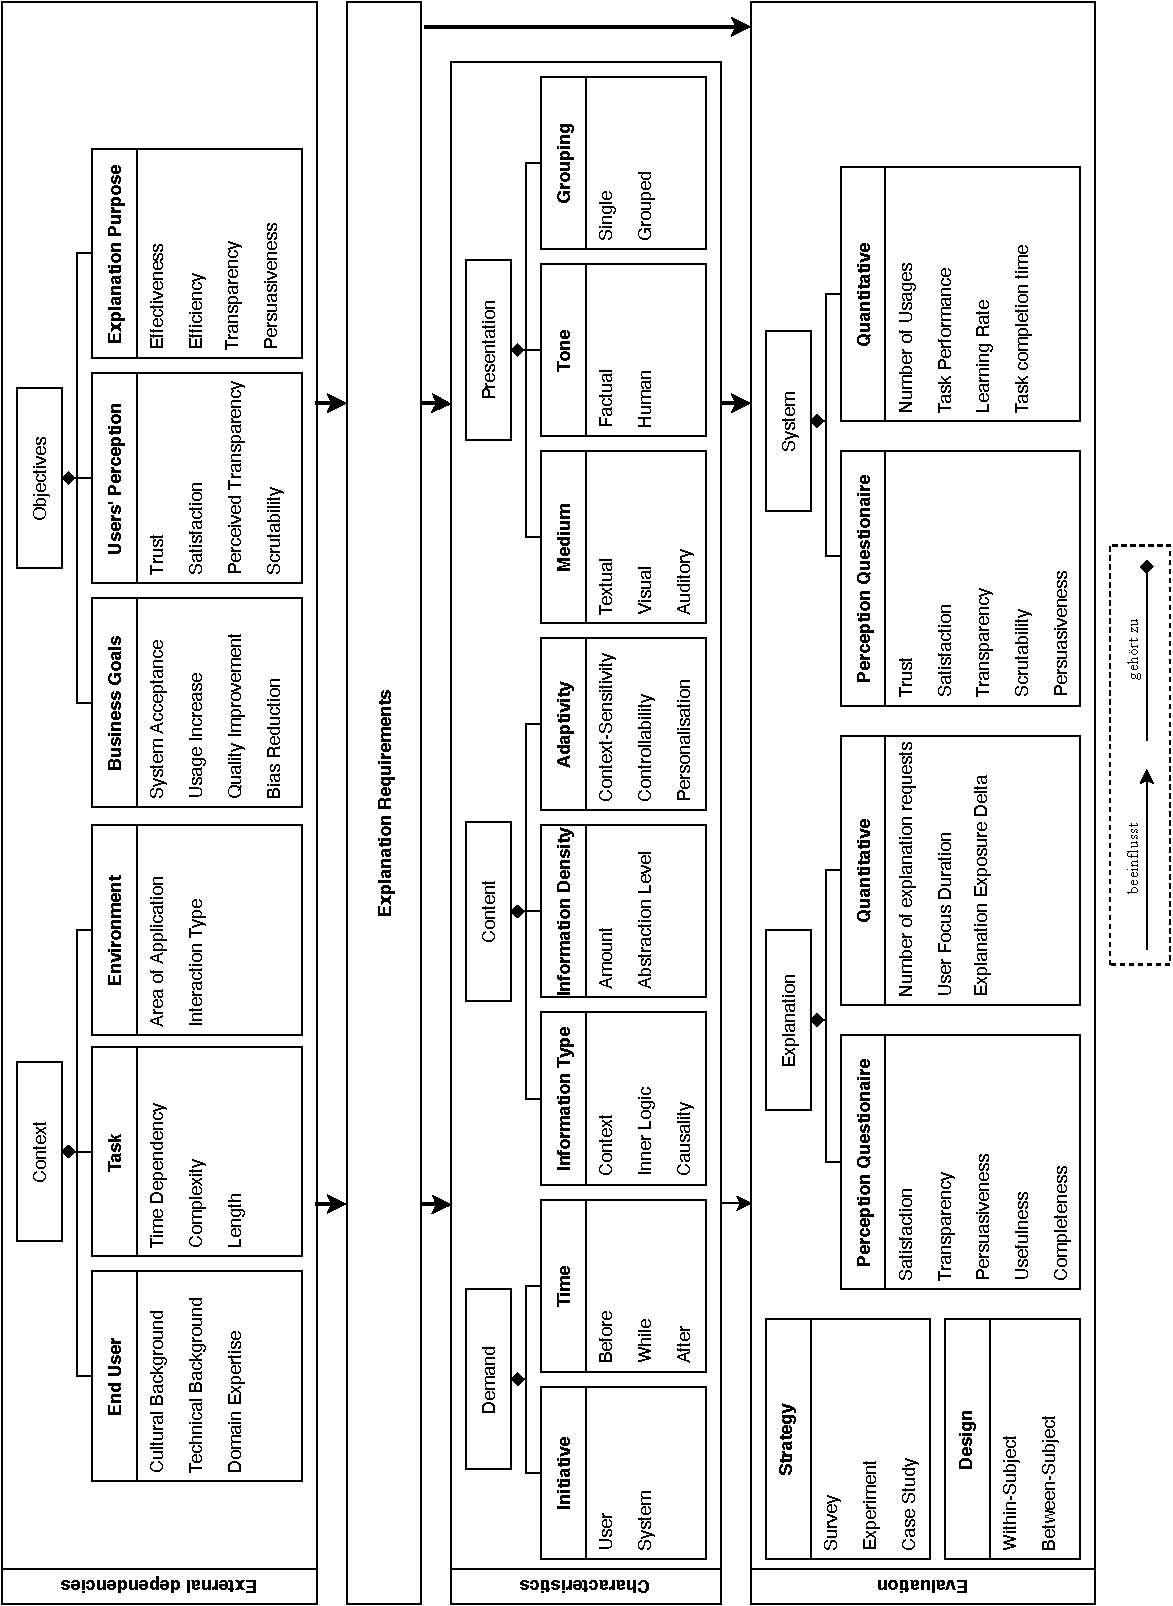
\includegraphics[width=\textwidth]{contents/05_model_description/res/model_complete_overview.pdf}
    \end{center}
    \caption{Übersicht über die Aspekte von Erklärbarkeit sowie dessen bekannte Ausprägungen aus der Literatur}
    \label{fig:model_overview_complete}
\end{figure}

\newpage